%TODO:
%	Formulation Section
%	Figures
%		Main diagram - break it up into pieces with just text
%		UVL three-axis diagram
%		Replace C with (pi,s)
%	Method:
%		Unprojection Consistency Loss
%		Texture Reality Loss

%TODO:
%	Formulation Section
%	Figures: Main diagram - break it up into pieces with just text
%	Figures: UVL three-axis diagram
%	Method:	Unprojection Consistency Loss
%	Method:	Texture Reality Loss


\newcommand{\Tab}{T_{A\rightarrow B}}
\newcommand{\Tba}{T_{B\rightarrow A}}
\newcommand{\pih}{\hat{\pi}}
\newcommand{\sh}{\hat{s}}
\newcommand{\ph}{\hat{p}}
\newcommand{\pis}{\pi,s} % pi and s pairs from domain A
\newcommand{\pish}{\pih,\sh} % pi and s pairs from domain A
\newcommand{\ppis}{(\pis)} %Parenthesized pis
\newcommand{\ppish}{(\pish)} %Parenthesized pis

\newcommand{\toB}{_{1\dots B}}
% \newcommand{\toBL}{_{1\dots B,\text{ } 1\dots L}}
\newcommand{\toBL}{_{1\dots B, 1\dots L}}
\newcommand{\toL}{_{1\dots L}}

\newcommand{\lUC}{\ell_{UC}}
\newcommand{\lTR}{\ell_{TR}}



%%%%%%%%%%%%BIG TODO::::
%%%%%% MAKE BATCH SIZE N INSTEAD OF B - B is a domain!


\documentclass{article}

% \usepackage{corl_2022} % Use this for the initial submission.
\usepackage[final]{corl_2022} % Uncomment for the camera-ready ``final'' version.
\usepackage{graphicx}
\usepackage{float}
\usepackage{amsfonts}
\usepackage{amsmath}
\usepackage[utf8]{inputenc}
\usepackage[T1]{fontenc}
\usepackage{array, booktabs, ragged2e}

%\usepackage[preprint]{corl_2022} % Uncomment for pre-prints (e.g., arxiv); This is like ``final'', but will remove the CORL footnote.

% \title{TRITON: Globally Consistent Sim-to-Real Transfer
\title{Neural Textures make Better Simulators

``I can't believe it's not real!" %Definitely gonna delete this lol
 %via Neural Textures
 }

\author{%
	Ryan Burgert \\
	Department of Computer Science\\
	Stony Brook University\\
	Stony Brook, NY 11794 \\
	\texttt{rburgert@cs.stonybrook.edu} \\
	% \And
	% Michael Ryoo \\
	% Department of Computer Science\\
	% Stony Brook University\\
	% Stony Brook, NY 11794 \\
	% \texttt{mryoo@cs.stonybrook.edu} \\
	\And
	Emma Burgert \\
	Ryan Burgert's Dog\\
}


\begin{document}
\maketitle

%===============================================================================

\begin{abstract}
	% Abstracts should be a single paragraph, between 4--6 sentences long, ideally. Gross violations will trigger corrections at the camera-ready phase.

	% Because of the 6 sentence limit, I've commented out some of the sentences...

	Unpaired image translation algorithms can be used for sim-to-real tasks, but most fail to generate temporally consistent results.
	% Because of this, the details or even identity of a particular object might change as it moves across a scene.
	We present a new approach that combines differential rendering with image translation to achieve temporal consistency over indefinite timescales.
%
	%TURNING TWO SENTENCES INTO ONE:
	% We call this algorithm TRITON (Texture Recovering Image Translation Network): an unsupervised, end-to-end, stateless sim-to-real algorithm.
	% Unlike previous techniques, TRITON leverages the underlying 3d geometry of input scenes by generating realistic-looking learnable neural textures.
	We call this algorithm TRITON (Texture Recovering Image Translation Network): an unsupervised, end-to-end, stateless sim-to-real algorithm that 
	leverages the underlying 3d geometry of input scenes by generating realistic-looking learnable neural textures.
%
	% These textures are projected onto the surfaces of input scenes, which are then fed through an image translation network to obtain the final outputs.
	By settling on a particular albedo for the objects in a scene, we ensure consistency between frames statelessly.
	Unlike previous algorithms, TRITON is not limited to camera movements - it can handle the movement of objects as well, making it useful for downstream tasks such as robotic manipulation.
	Our experiments show that in addition to achieving higher temporal consistency, the translations are closer to ground truth photographs than previous techniques.

\end{abstract}

% Two or three meaningful keywords should be added here
\keywords{sim to real, image translation, differentiable rendering} 

%===============================================================================

\section{Introduction}
	

I introduce you to TRITON. The rest of the introduction text goes here; I've commented out my old incomplete introduction.

% TODO: Note that the simple input of UVL, or an RGB neural texture, means any simulator should be plug-and-play with this algorithm.

% Recently, several sim-to-real algorithms have come out that are based on image-to-image translation. [Citations]
% These are used for training robots using pixel-based reinforcement learning.
% They demonstrated that better image translation algorithms yielded notable improvements in robotic benchmarks.
% At the same time, there is a lot of research on differentiable rendering,
% a topic which produced papers such as NERF which attempt to capture 3d representations of the real world.
% However, most of these approaches are either supervised or involve only camera movements [citations].
% One paper that came out recently combined both image translation and differentiable rendering in an unsupervised manner to create view-consistent models of human organs [citation].
% This paper too, though, was limited to only camera movements.

% This algorithm unlocks a new capability: learning textures to match photos for given 3d models without supervision.

% The motivation for this paper is to create a temporally consistent sim-to-real image translation algorithm that will look the same from multiple camera angles simultaneously, keeps all semantic details 
% [[I'll finish this later... let's work on the meat of the paper first...]]

		

%===============================================================================


\section{Formulation}
\label{sec:data}





% TODO: Describe what UVL is ; 
% Formulate the setting: What our inputs are and the targets are and what we learn (a neural texture function) and how we can take advantage of it for robotic learning.
% Don't go into details; just say 'its a black box function'

% TODO: Add UV to the fourier feature diagram.

% TODO: Create subfigures with subcaptions. 
% 2a: Nothing but UVL=UV+L
% 2b. 3d uvl axis to texture pack (drew on whiteboard)
% 2c. Skip over the translation network and show a pretty robot arm picture

% This is the formulatoin section; not data section. Dont talk about how many photos we use etc. 

% JUST IN CASE THINGS ARE ERASED:
% We learn neural texture corresponding to each object, where each texture is represented as a function mapping... 
% The idea is to learn object textures as a set of continuous functions from a set of (unlabeled) real images, and use them to generate realistic images.
% Given a 3D structure of the scene represented with a UVL image, the learned neural textures will translate them into a realistic image.
% When used for the robot learning, this enables learnable, realistic sim2real of robot training images.

% IN THE INTRODUCTION: How we're using a neural neural network network texture. Also in related works.

% TODO: Replace neural texture in figure 3 with axis, and treat it as a function that takes UV in with an arrow pointing to it.

% BREAK IT DOWN APPROACH:
% Don't have any pictures. Have breakdown where we add new things in multiple figures.
% First figure: Just image translation. 
% Seconf:
% Third:
% Etc...


\begin{figure}[H]
	\begin{center}
		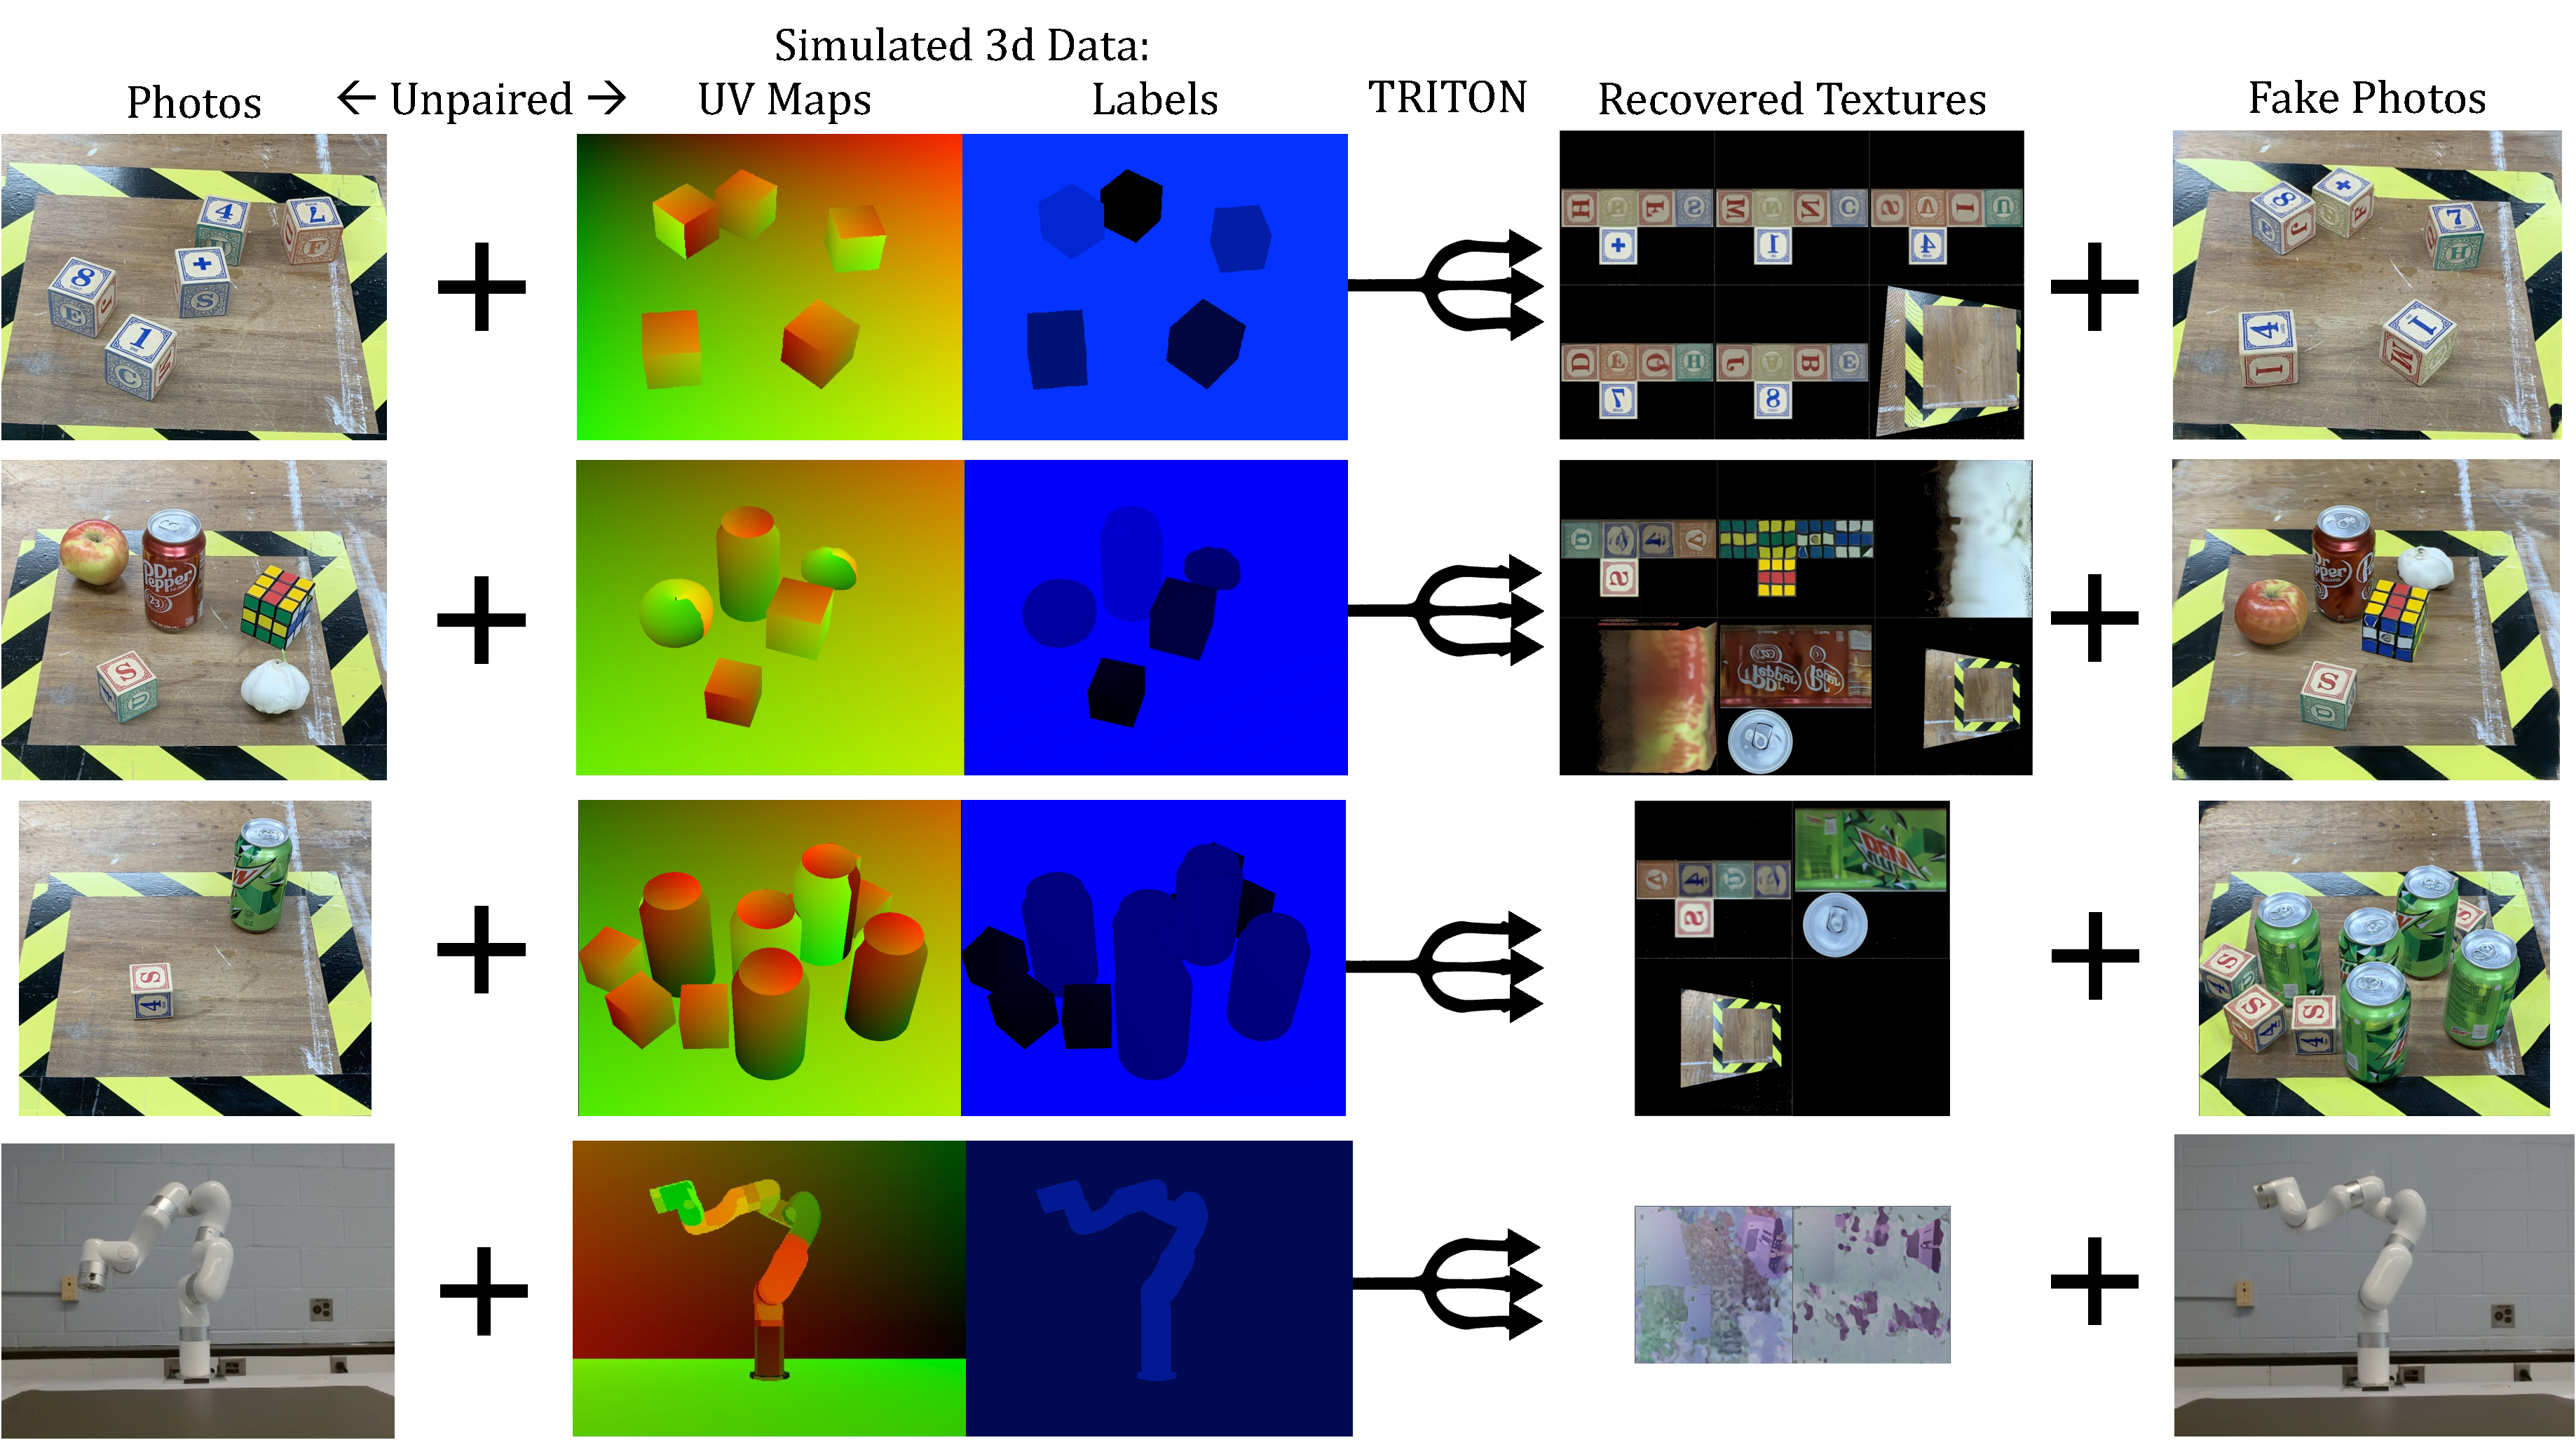
\includegraphics[width=400pt]{../images/first_diagram.pdf}
	\end{center}
	\caption{
		This is an overview of what TRITON accomplishes.
		TRITON learns the textures of 3d objects to help translate simulated images into photographs. It does this with unpaired data. Each row is a different dataset.
		}
	\label{fig:uvl_explanation}
\end{figure}




\begin{figure}[H]
	\begin{center}
		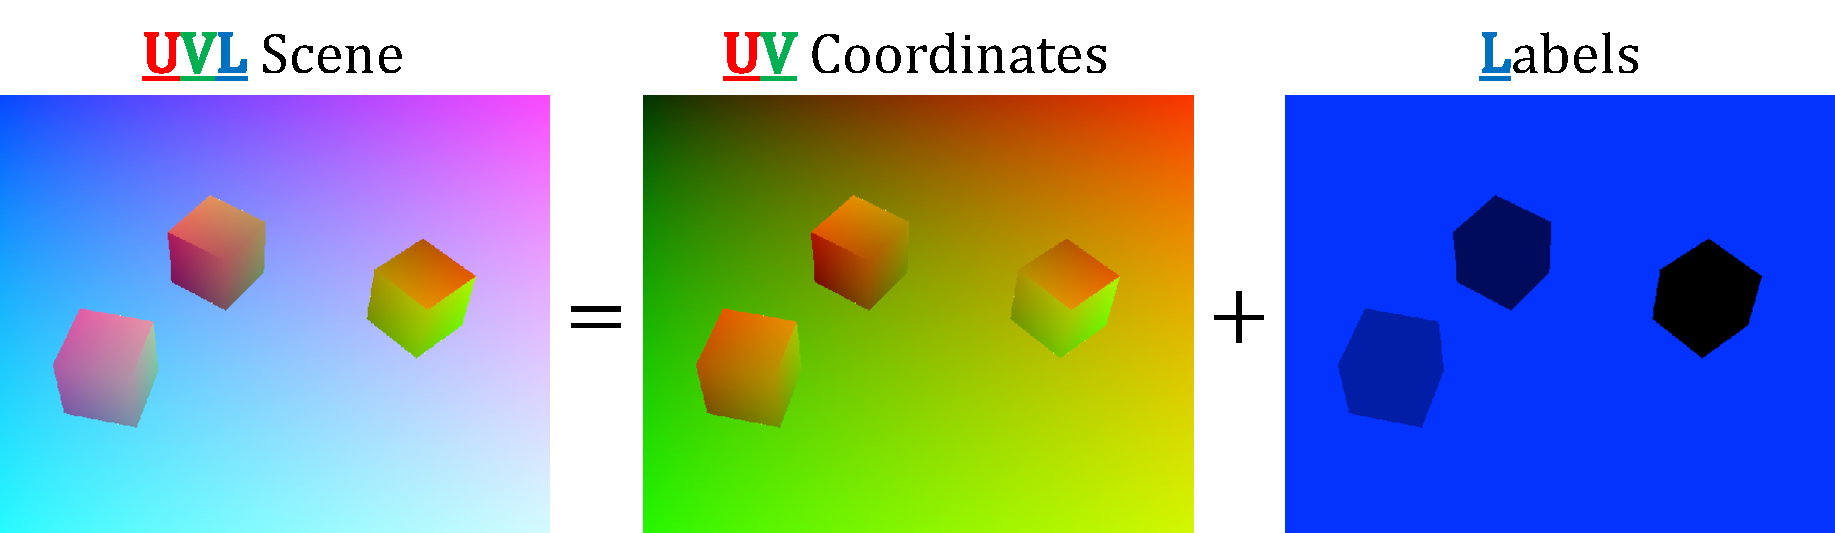
\includegraphics[width=400pt]{../images/uvl_explanation_minimal.pdf}
	\end{center}
	\caption{
		% This diagram shows the purpose of a UVL image.
		A UVL scene is an image that has three channels: RGB.
		R and G are used for U and V, and B is used for L.
		L stands for Label, and determines which part of the synthetic image will get which texture.
		The U and V coordinates correspond to positions on each texture,
		telling it how to project the textures onto the 3d objects represented in the UVL scene.
		The darkest shade of blue corresponds to the 1st texture, and the next darkest shade of blue corresponds to the 2nd texture etc.
		}
	\label{fig:uvl_explanation}
\end{figure}



% In this paper, we'll mostly focus on a hand-collected dataset that involves three alphabet blocks that are moved across a table.
% Alphabet blocks were chosen because they all have the same geometry (a cube), but have very distinct semantic textures that will make temporal inconsistency obvious to the human eye.
% This dataset is analogous to data that would be collected for a third-person robotic grasping task.
% However, other objects (such as cans of soda, apples, cloves of garlic, etc) are also for generating other results in this paper. ((TODO: Detail the five object tests and five cube tests and other stuff like shiny cans etc)).

% There are two components to this dataset: Simulated data in the form of UVL scenes, and photographs.
% The camera in the simulation is positioned in approximately the same place as the real camera, with approximately the same field of view.
% In both domains of this dataset, the camera never moves. Instead, the objects are randomly positioned and rotated on the table.
% In both the simulation and in real life, these objects are randomly translated along the x and y-axis of the table, as well as rotated on the z-axis.

% There are 200 photographs in this dataset, and they are recorded as RGB jpg images.
% There are 3000 synthetic images in this dataset, in the form of UVL images.
% These UVL images are also encoded as RGB images, but provide information about the geometry of a scene.
% UVL images are composed of both a UV map and a label map and are summarized in figure \ref{fig:uvl_explanation}.
% To avoid positional rounding errors, UVL images are encoded as EXR files: an image format that supports floating-point values.

% The pixels in a UVL image are visualizable in RGB space because, like RGB images, each pixel is a vector with 3 values. The first two channels, U and V, are floating point values between 0 and 1. The L channel is also a floating point value between 0 and 1, it has a second meaning. There are only a finite number of label values (corresponding to the number of learnable textures). The rank of a particular L value is used to index these textures.

% In the three-cube dataset we have 4 textures, and UVL scenes contain label values $l \in [\frac{0}{3}, \frac{1}{3},\frac{2}{3}, \frac{3}{3}]$. A pixel in a UVL scene $l=\frac{2}{3}$ will get indexed to the third texture, because $\frac{2}{3}$ is the third smallest label value.

% %===============================================================================

% Domain A and B
% p hat
% s hat

\section{Method}
\label{sec:method}


\begin{figure}[H]
	\begin{center}
		% \includegraphics[width=400pt]{../images/main_diagram_condensed.pdf}
		\includegraphics[width=400pt]{../images/main_diagram_condensed_with_domains.pdf}
	\end{center}
	\caption{
		% We use differentiable rendering paired with unpaired image translation to consistently= transform synthetic scenes into realistic images.
		% To ensure all objects look consistent in different positions and views, we learn the albedo of each object's surface by using a learnable latent texture.
		% This texture is parametrized as an image generated by an MLP which is fed Fourier features, as shown in figure \ref{fig:learnable_textures}.
		% $B$ is the batch size, and $L$ is the number of different labels (which is also the number of learnable textures).
		This figure is an overview of how TRITON works, showing all submodules and losses.
		Inputs are on the left, and outputs are on the right.
		The dashed arrows indicate losses between nodes.
		Although $\pi\toB$ and $\ph\toB$ look similar, they are not identical - $\lTR$ encourages them to look as similar as possible.
		% $\pi$ is simply projected textures, whereas $\hat{p}$ has been run through an image translator, allowing it to have shadows and specularities.
		% TODO: Come up with a tour of this diagram in this caption. Also maybe make it larger?
		% TODO: Use variables instead of 3,4
		% TODO: Make the text larger and easier to read
		% TODO: Simplify the diagram?
	}
	\label{fig:main_diagram}
\end{figure}


	In this section, we describe how TRITON works to translate images from domain A (simulation) to domain B (photos) while maintaining surface consistency. 
	TRITON has four main components: a neural texture, an image translator, and two surface consistency losses.
	\begin{enumerate}
		\item{
			Neural Textures $\tau\toL$: Given an input scene $s$ depicting 3d objects with labels $1\dots L$, we project learnable RGB textures $\tau\toL$ to their surfaces to obtain projection $\pi$. 
			These neural textures are represented implicitly by a neural network that maps UV values to RGB values, and are learned jointly with the image translator.
			\begin{equation}
				\pi=\tau\toL(s)
			\end{equation}
			We then concatenate the scenes with the projections channelwise to obtain images from domain A: $\ppis \in A$.
		}
		\item{
			Bidirectional Image Translator $T$: $\Tab$ translates images from domain A to domain B, and $\Tba$ translates images from domain B to domain A.
			\begin{equation}
				\ph=\Tab(\pis)\ \ \ \text{ and }\ \ \ \ppish=\Tba(p)
			\end{equation}
			$T$ is a variation of MUNIT, and inherits adversarial losses $\ell_{adv}$, as well cycle consistency losses $\ell_{cyc}$ and reconstruction losses $\ell_{rec}$.
		}
		\item {
			Unprojection Consistency Loss $\lUC$: To keep the object surfaces consistent between a batch of $B$ scenes, we impose a pixel-wise similarity loss between these surfaces by warping them back into a common texture space using the UV and label values contained in the original scene. 
			\begin{equation}
				u\toBL=\text{unproject}(\ph\toB,s\toB)\ \ \ \text{ and } \ \ \ \lTR \Rightarrow u_1 \approx u_2 \dots \approx u_B
			\end{equation}
		}
		\item{
			Texture Realism Loss $\lTR$: To encourage the neural textures to look as realistic as possible, we try to make the projections look like the final output. 
			\begin{equation}
				\lTR \Rightarrow \pi \approx \ph
			\end{equation}
			As it turns out, $\lTR$ is sufficiently powerful loss to generate surface-consistent translations even without $\lUC$, although the results are better when both losses are used.
		}
		
	\end{enumerate}

\subsection{Neural Texture and Projection}

	\begin{figure}[H]
		\begin{center}
			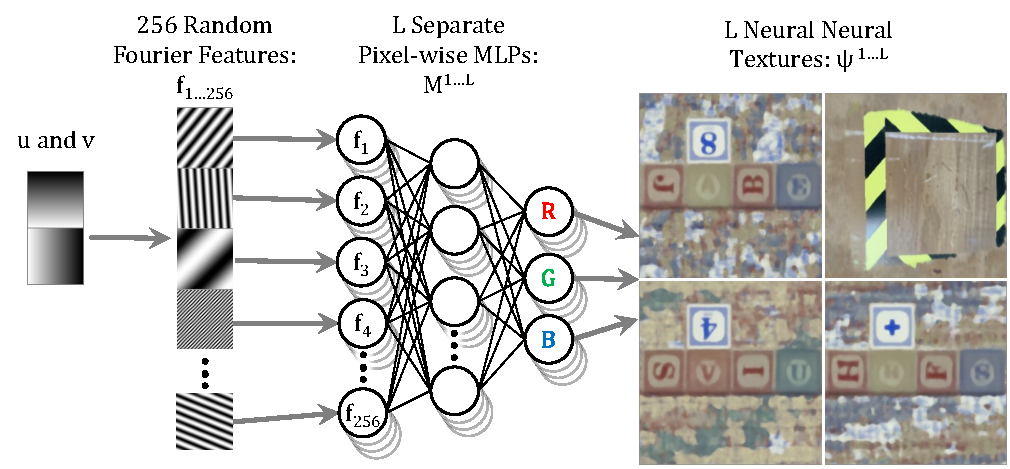
\includegraphics[width=300pt]{../images/learnable_textures.pdf}
		\end{center}
		\caption{
			This figure illustrates how the neural textures are calculated in figure \ref{fig:main_diagram}. They are fully differentiable, and represented continuously along the texture's U and V axes using fourier feature networks.
		}
		% For each texture, there is a separate Fourier feature network (Fourier features fed into a pixel-wise MLP) that will take in Fourier features as inputs, and output an RGB image using the method described in \citet{fourier_feature_networks}.
		% We found this method gave better results than storing each differentiable texture as a raster matrix of pixels, as well as being faster to train.
		% During inference, you can store the results of this MLP as a raster image of arbitrarily large resolution, saving both time and VRAM.
		\label{fig:learnable_textures}
	\end{figure}

	TRITON's neural texture module lets it  of objects, and thus take advantage of 3d geometric priors. By learning this texture, we can encode features directly onto the surfaces of the 3d objects in a scene, which the image translation module uses to maintain visual consistency between states and viewpoints.

	Given a batch of $B$ UVL Scenes $s_{1\dots B}$ with $L$ different label values, we project $L$ different neural textures $\tau_{1\dots L}$ onto that scene; obtaining projections $\tau_{1\dots B}$. This projection mechanism is illustrated in figure \ref{fig:uvl_explanation}.

	These neural textures are not stored in raster form during training. Instead, as illustrated in figure \ref{fig:learnable_textures}, they're paramaterized by pixel-wise fourier feature networks \cite{fourier_feature_networks} that take in UV coordinates and returns RGB colors. During inference, however, these textures are rasterized to save both time and video memory.
	
	Each neural texture $\tau_i$ is a function consisting of two components: a multi-layer perceptron $M_i$ and a static set of 256 random spatial frequencies $f_{1...256}$. 
	Given a two-dimensional $uv$ vector, the spatial frequencies are used to generate a high dimensional embedding used as input for the MLP.
	\begin{equation}
			\tau_i(uv) = 
			\
			M_i\left(\left[
				\sin f_1 uv, \ 
				\cos f_1 uv, \ 
				\sin f_2 uv, \ 
				\cos f_2 uv, \ 
				\dots \ 
				\sin f_{256} uv, \ 
				\cos f_{256} uv \ 
			\right]\right)
	\end{equation}
	where $uv$ and $f_i \in N_{ormal}(\mu=0,\ \sigma=10)$ are two dimensional vectors,
	 $f_i uv$ represents their dot product, 
	%  $rgb$ represents a 3d color vector,
	 and $M_i$ maps a $uv$ embedding to an $rgb$ color value:
	 $M_i: \mathbb{R}^{256} \rightarrow \mathbb{R}^3$.
	Note that there is nothing special about 256 or 10: these hyperparameter values just happen to work nicely.
	
	A particular neural texture $\tau_i$ uses maps $uv \rightarrow rgb$. Similarly, the set of textures $\tau_{1\dots L}$ maps uvl values to rgb values: $\tau_{1\dots L}(uvl)=\tau_l(uv)$ where $uvl$ is the concatenation of a $uv$ vector with a label $l \in 1\dots L$.
	
	In practice, we found that TRITON learns faster with fourier-feature textures than raster textures. The trained fourier-feature textures also exhibit less noise than its raster counterparts. We think this is because they don't suffer as muchIt cfrom aliasing artifacts in the UV maps, where the loss gradient might skip over pixels in texture-space when the UVL scene is zoomed out too far or raster resolution is too high. Case in point: if you have a raster texture with very high resolution, the loss gradient is less likely to be passed to a given texel because the chance that a given UV value in a scene will be rounded to that pixel's coordinates is very small.

	% UV Map projection
	% We use an RGB texture, parametrized by an MLP taking fourier features as an input.
	% We use a separate MLP for every texture. 



\subsection{Image Translation}
\label{sec:image_translation}

\begin{figure}[H]
	\begin{center}
		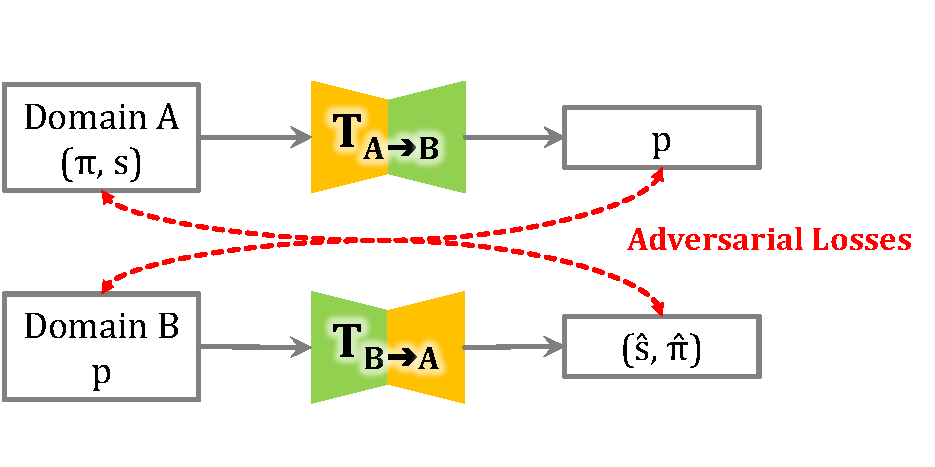
\includegraphics[width=200pt]{../images/module_translator.pdf}
	\end{center}
	\caption{
		A subset of figure \ref{fig:main_diagram} focusing on the image translation module $T$.
	}
	% For each texture, there is a separate Fourier feature network (Fourier features fed into a pixel-wise MLP) that will take in Fourier features as inputs, and output an RGB image using the method described in \citet{fourier_feature_networks}.
	% We found this method gave better results than storing each differentiable texture as a raster matrix of pixels, as well as being faster to train.
	% During inference, you can store the results of this MLP as a raster image of arbitrarily large resolution, saving both time and VRAM.
	\label{fig:learnable_textures}
\end{figure}


% TO PUT IN FORMULATION:
% The simulation domain A (UVL maps concatenated to their texture projections) has 6 channels, whereas the real image domain B (photographs) has 3 channels. An element of A is $\ppis \in A$ and $p \in B$.
% $p \in B$ is a batch of real photos,
% and $\ppis\in A$ is a batch of simulated projection/uvl scene concatenations. 

% TODO: Why doesn't citep work? The references don't show the authors names...it used to work...did I mess up example.bib?

% TODO: Get rid of the variable "C" and replace it with $\ppis$

% TODO: Is l2 loss capitalized or lower case?

Our image translation module, $T$, is based on the image translation module used in \citep{surgical_video_translation}, which is a based on a variant \cite{surgical_image_translation} of MUNIT \cite{munit}. The main differences between our image translation model and MUNIT are that our style code is fixed making it unimodal, noise is injected into the latent codes during training to prevent overfitting, and we use a different image similarity metric. During inference however, this intermediate noise is removed and our image translation module is completely determinstic. Apart from these differences, our image translation module has the same loss formulations and generator/encoder/discriminator network architectures as MUNIT. 

$T$ is a bidirectional image translation module, and has two translation directions. $\Tab$ translates sim to real (aka domain A to domain B), and $\Tba$ translates real to sim (aka domain B to domain A).

MUNIT translates images by encoding both image domains into a common latent space, then decoding them into their respective domains.
In our translation module, we define fake photos $\ph = \Tab(\pis) = G_B(E_A(\pis))$ and fake projection/uvl scenes $\ppish = \Tba(p) = G_A(E_B(p))$
	where $E_A, E_B, G_A, G_B$ are encoders and generators for domains A and B respectively.
% We also define the outputs of these translators as fake photos $\hat{p} = T_{A\rightarrow B}(\pis)$ and fake projection/uvl scenes $(\hat{\pi},\hat{s}) = T_{A\rightarrow B}(\pis)$.

% TODO: Choose one of the three equation representations. Which is best? The next paragraph will look less ugly when the equations are shorter.

To ensure cycle consistency, we have an image similarity loss $\ell_{cyc}$ to ensure
% $c \approx G_A(E_B(G_B(E_A(\pis)))) = T_{B\rightarrow A}(T_{A\rightarrow B}(\pis)) = T_{B\rightarrow A}(\hat{p})$
$\ppis \approx T_{B\rightarrow A}(\hat{p})$
and vice versa
% $p \approx G_B(E_A(G_A(E_B(p)))) = T_{A\rightarrow B}(T_{B\rightarrow A}(\pis)) = T_{A\rightarrow B}(\hat{c}) = T_{A\rightarrow B}(\hat{\pi},\hat{s})$. 
$p \approx T_{A\rightarrow B}(\hat{\pi},\hat{s})$.
%I only want to use one of the two representations; either using T_AB or GA(EB) etc. Which one should I use?
We also impose an image similarity loss $\ell_{rec}$ to ensure that $\ppis \approx G_A(E_A\ppis)$ and $p \approx G_B(E_B(p))$, which is effectively an autoencoder loss. 
In addition, we also have content similarity loss $ \ell_{con}$ to make 
$E_A(\pis) \approx E_B(\ph)$ and $E_A(p) \approx E_A(\pish)$.
% $E_A(\pis) \approx E_B(\Tab(\pis))$ and $E_A(p) \approx E_A(\Tba(p))$.

Our similarity losses are the sum of L2 distance and negative multi scale structural image similarity (MS-SSIM), introduced in \citep{msssim}. For our purposes, MS-SSIM is a metric that measures the similarity of two BCHW tensors on a scale from 0 to 1. Given two tensors $x$ and $y$, their similarity loss is $\mu\left((x-y)^2\right) - \text{msssim}(x,y)$. 

We also have adversarial losses $\ell_{adv}$ that come from two discriminators $D_A$ and $D_B$, targeting domains A and B respectively. They use the LS-GAN loss introduced in \citep{lsgan}.

In total, the loss for the image translator module $T$ is $\ell_T=\ell_{cyc}+\ell_{rec}+\ell_{con}+\ell_{adv}$.



% NOTE: THe other paper \citep{surgical_video_translation} didn't do into this much detail; instead putting most of these losses in teh appendix. I think we can cut this down? I'll check with michael first...right now I'll include everything.




\subsection{Unprojection Consistency Loss}
\label{sec:unprojection_consistency_loss}

\begin{figure}[H]
	\begin{center}
		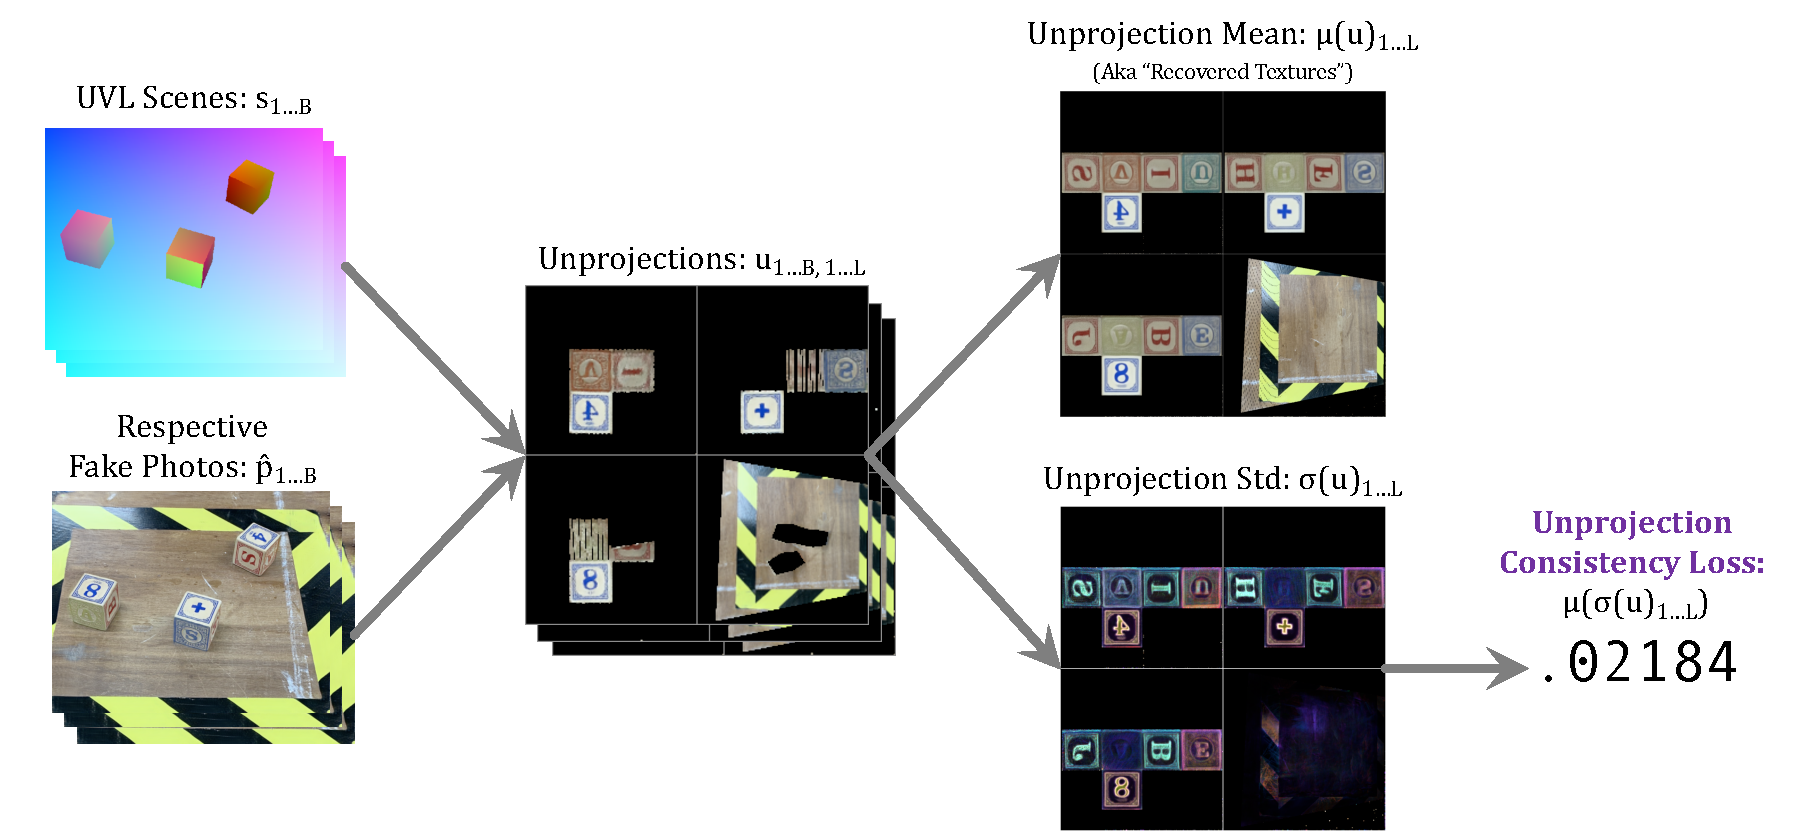
\includegraphics[width=400pt]{../images/unprojection_consistency_loss.pdf}
	\end{center}
	\caption{
		This is the unprojection consistency loss used in figure \ref{fig:main_diagram}.
		The Unprojection Mean and Reprojection nodes are not used in any losses, and help to illustrate the next section \ref{sec:texture_realism_loss}.
		% After calculating fake photos $\hat{p}_{1...B}$ from UVL scenes $s_{1...B}$ as seen in figure \ref{fig:main_diagram}, 
		% we can unproject fake photos $\hat{p}_{1...B}$ back into texture space to obtain $u_{1...B,\ 1...L}$ .
		% If the fake photos display consistent textures along their 3d surfaces, then the unprojected textures should be similar.
		% We can measure this similarity by taking the per-channel standard deviation of these unprojections, aka $\sigma(u)$, then averaging the result.
		% When the fake photos display similar surfaces, the unprojections will be similar making the unprojection consistency loss low.
		% Additionally, we can also calculate the average unprojection, which is useful for visualization purposes (it will look blurry if $\hat{p}$ is inconsistent).
	}
	\label{fig:unprojection_consistency_loss}
\end{figure}

To maintain surface consistency, we sample a random batch of UVL scenes $S\toB$, and translate them into $\ph\toB$.
Using geometric knowledge of the scene encoded in $S\toB$, we individually unproject each $\ph_i \in \ph\toB$ back into texture space, to obtain $B$ sets of $L$ unprojected textures $u\toBL$.
We then use the per-pixel, batch-wise standard deviation of the unprojections as unprojection consistency loss $\lUC = \sigma(u\toBL)\toL$.
This loss observes how different these unprojections are from one another, and thus how different the object surfaces appear between translations. 

Intuitively, if $\lUC$ were $0$, it would mean the object surfaces in translations $\ph$ appear exactly the same in every scene.

This loss is a fairly intuitive and effective way to maintain surface consistency. There are some caveats, however.
In order to produce a standard deviation greater than $0$, we must have a batch size greater than $1$.
Furthermore, environments that rarely show a particular region of a surface will rarely have $\lUC$ applied to that region because they're unlikely to show up twice in the same batch.
For this reason, $\lUC$ is most useful with large batch sizes.% because observing the same surface in multiple elements of a batch becomes more likely as the batch size increases. 
But because video memory limits our batch sizes, first-person environments might be more of a challenge for $\lUC$ - particularly when exploring multiple rooms (a task we haven't done though - should I mention this?)

To michael: Should we mention these caveats in this section, or mention them in the texture realism loss section? That section addresses all of these issues...
 
% Also, you have to get lucky - two scene pictures have to show the same side of a cube for example. First person scenarios would be even worse.

\subsection{Texture Realism Loss}
\label{sec:texture_realism_loss}

\begin{figure}[H]
	\begin{center}
		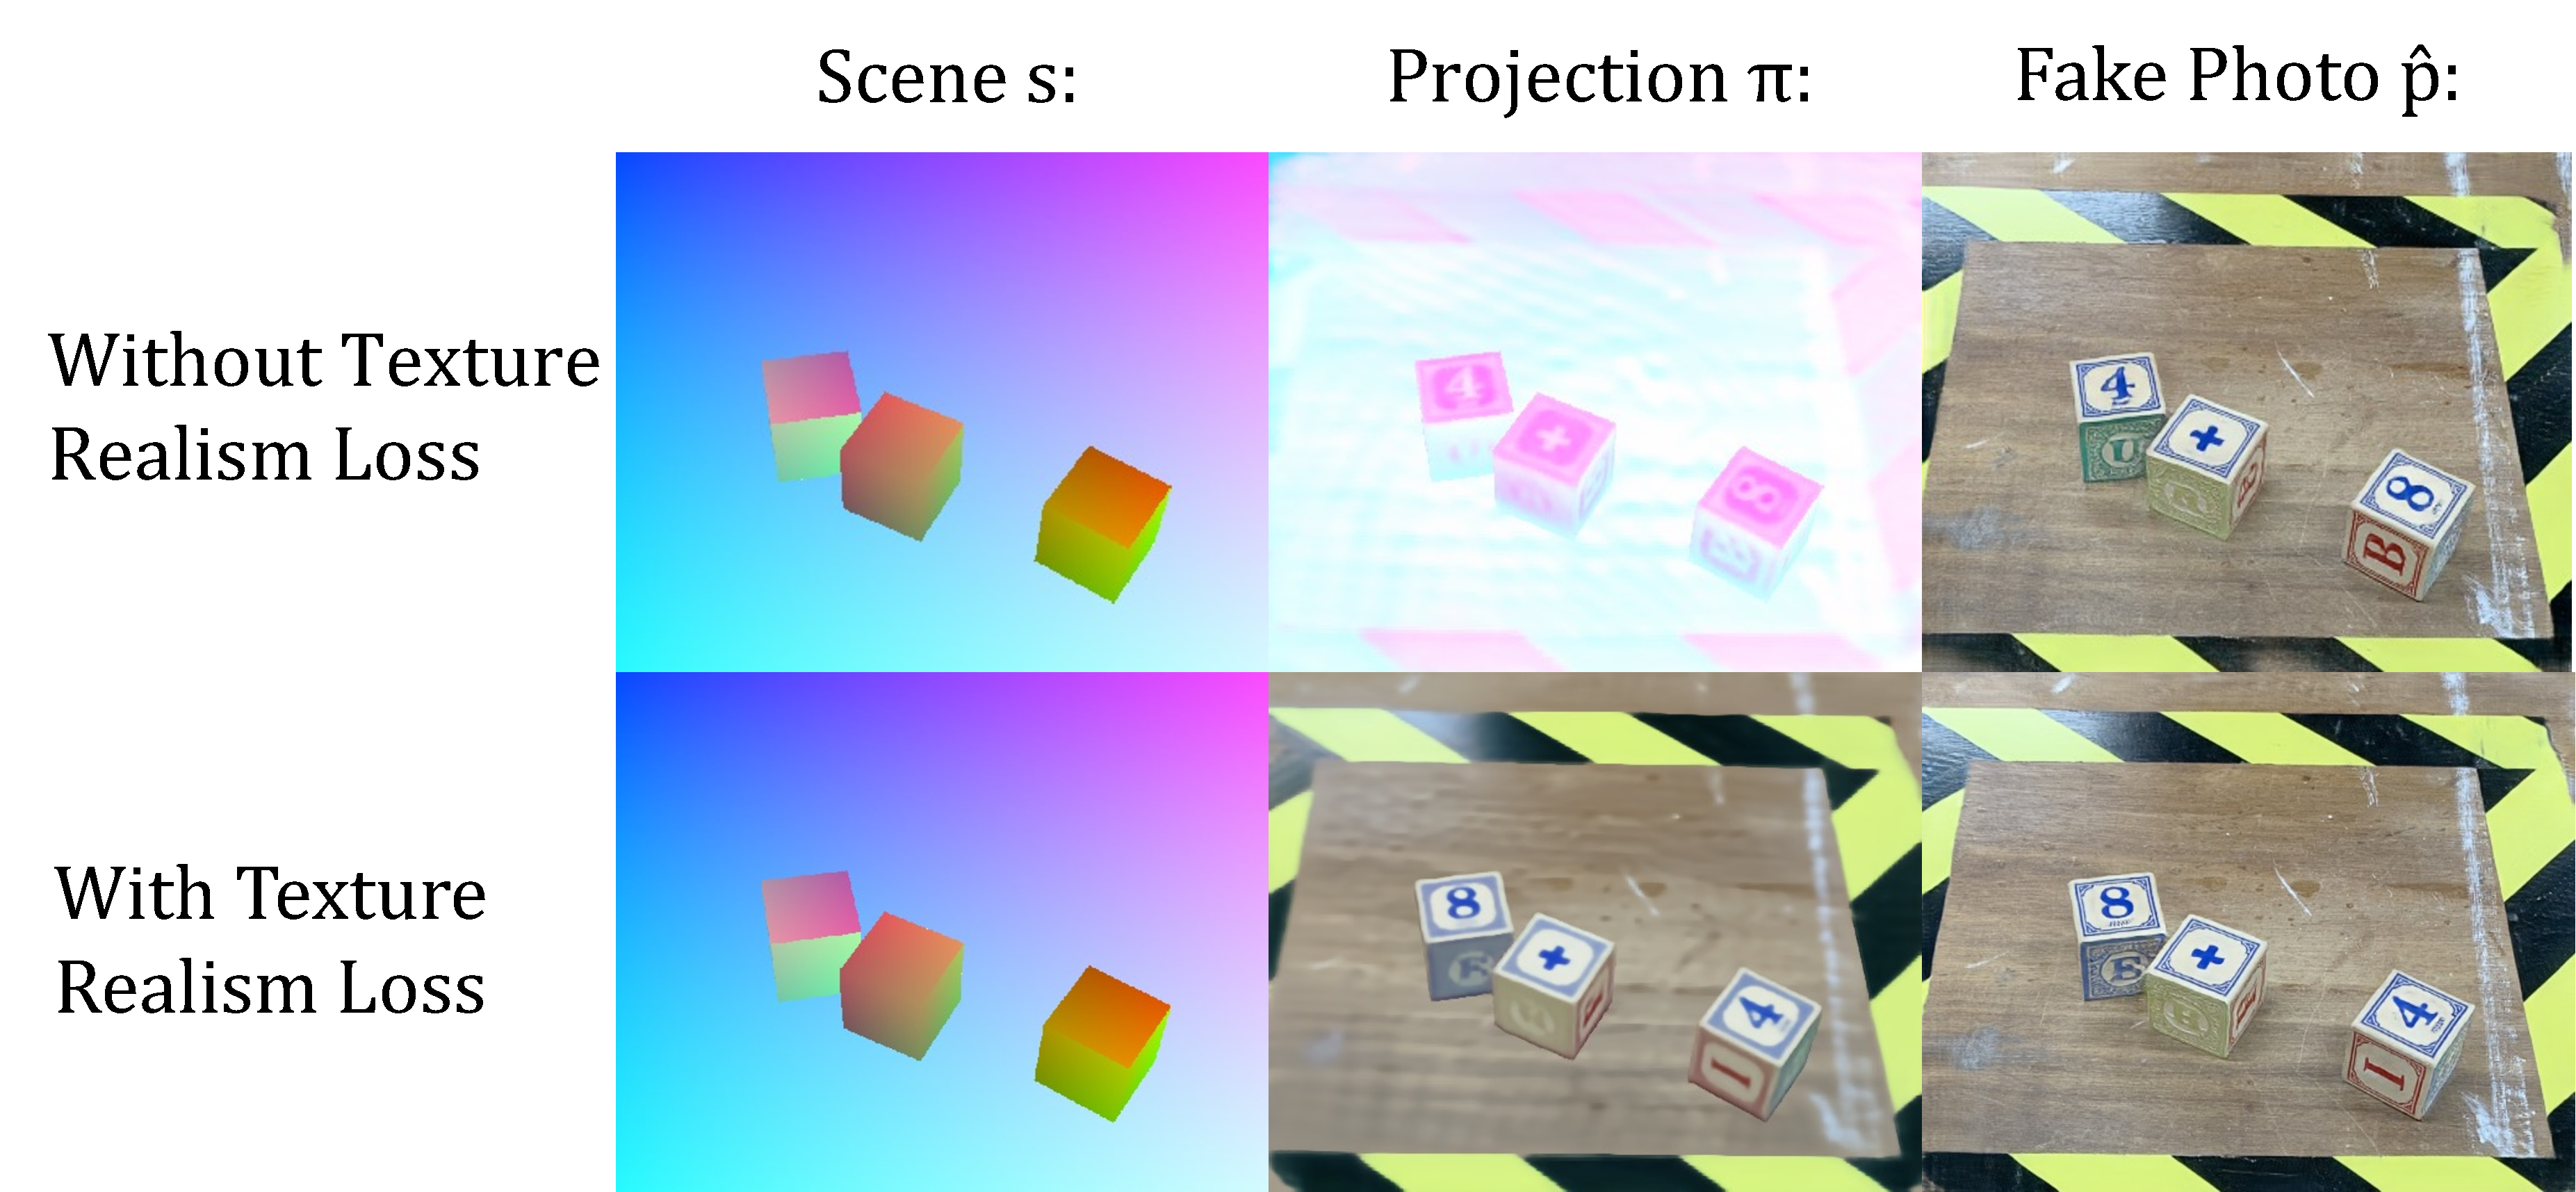
\includegraphics[width=250pt]{../images/texture_realism_ablation.pdf}
	\end{center}
	\caption{
		The neural texture looks more realistic with texture realism loss enabled. Note that the blocks show different letters because of different initializations and the symmetry of a cube - both solutions are valid texture assignments. 
	}
	\label{fig:texture_realism_ablation}
\end{figure}

We can improve the translation results by forcing the neural texture to look realistic, instead of allowing it to have arbitrary colors.
To do this, we add a texture realism loss $\lTR$.
$\lTR$ is an image similarity loss that makes $\pi$ look like its translation $\hat{p}$.
In other words, $\lTR$ makes the neural texture more realistic by making the neural texture projections more realistic.

So far, we've taken an image translator $T$ and added neural textures $\tau$ and a surface consistency constraint $\lUC$. 
If we wanted to, could stop here - those formulations are sufficient to produce consistent sim-to-real translations.
However, we can improve this further.

% Up until now we have not put any constraints on this neural texture. 
Without $\lTR$, $\tau$ can look wildly different each time you train it.
As seen in the top row of figure \ref{fig:texture_realism_ablation}, the neural texture looks very unrealistic - the colors are completely arbitrary.
After adding $\lTR$ though, $\pih \approx \ph$, and $\tau$ to represents the albedo of the surfaces in the scene.
The image similarity loss used in $\lTR$ is calculated the same way image similarity losses are calculated in section \ref{sec:image_translation}: L2 loss minus MSSSIM.

As it turns out, $\lTR$ is sufficient to ensure surface consistency without $\lUC$, though using both yields better results than either one alone. 
For an explanation of why this is the case, see the appendix \ref{sec:texture_realism_theory}.
There are some advantages to using $\lTR$ alone though: when just using $\lTR$ you can use batch sizes as small as $B=1$, allowing you to save video memory. 
Using $\lTR$ is also more numerically stable, as you no longer have to worry about whether the same surfaces are seen across multiple scenes in a batch.

% We introduce a new loss, called texture realism loss that fixes this: $\lTR$ is an image similarity loss that encourages $\pi \approx \ph$.
% This loss forces the neural texture to approximate the albedo of the surfaces in a scene.

% These images could be regularized so that they're the same every time.
% 
% To do this we put a penalty on the latent texture that makes it $\pi$ look like its translation $\hat{p}$. 
% 
% We use l2 and msssim losses to do this.
% 
% This helps improve the translations.
% 
% There are some advantages over unprojection consistency though: 
% smaller batch sizes (even a batch size of 1, which UC cant do),
% you don't have to get lucky (the more chaotic, or even the more zoomed in a dataset becomes the less likely there is to be any collisions)

\subsection{Color Loss}

TRITON is very robust to geomtric imperfections. However, sometimes it takes this a bit too far - it can overfit textures onto the wrong objects and still maintain consistency.
In one example, it manages to map an apple texture onto a cube. 

To help TRITON correctly match textures to objects, we introduce a small amount of supervision by adding a color loss. I'm going to stop writing this because I don't know if I even want to keep this in the paper...you can achieve the same result by running the algorithm multiple times, and so its not strictly nessecary.

ASK MICHAEL: I'd rather not mention this entire section and run out the page limit...it's not very important, and not used in the robot experiments. It's only used in the experiment with the five items including the apple. Can we add it to the appendix instead?

%===============================================================================


\section{Results}

\subsection{Data}

Here I detail the datasets used in the results section. 
Every dataset has two sets of images: UVL scenes and photographs. They are all unpaired, and have RGB values ranging from 0 to 1.

The first dataset to mention is the three-block dataset.  
It has 300 photos and 2000 UVL scenes. It features a table with three alphabet blocks on a table, which are randomly translated along the X and Y axes and rotated randomly along the Z axis. Each photograph features these three cubes with a random position and rotation.

[[Insert photographs and UVL maps here; a digram showing each dataset we describe here and 1 or two samples of each domain in each dataset]]

% In this paper, we'll mostly focus on a hand-collected dataset that involves three alphabet blocks that are moved across a table.
% Alphabet blocks were chosen because they all have the same geometry (a cube), but have very distinct semantic textures that will make temporal inconsistency obvious to the human eye.
% This dataset is analogous to data that would be collected for a third-person robotic grasping task.
% However, other objects (such as cans of soda, apples, cloves of garlic, etc) are also for generating other results in this paper. ((TODO: Detail the five object tests and five cube tests and other stuff like shiny cans etc)).

% There are two components to this dataset: Simulated data in the form of UVL scenes, and photographs.
% The camera in the simulation is positioned in approximately the same place as the real camera, with approximately the same field of view.
% In both domains of this dataset, the camera never moves. Instead, the objects are randomly positioned and rotated on the table.
% In both the simulation and in real life, these objects are randomly translated along the x and y-axis of the table, as well as rotated on the z-axis.

% There are 200 photographs in this dataset, and they are recorded as RGB jpg images.
% There are 3000 synthetic images in this dataset, in the form of UVL images.
% These UVL images are also encoded as RGB images, but provide information about the geometry of a scene.
% UVL images are composed of both a UV map and a label map and are summarized in figure \ref{fig:uvl_explanation}.
% To avoid positional rounding errors, UVL images are encoded as EXR files: an image format that supports floating-point values.

% The pixels in a UVL image are visualizable in RGB space because, like RGB images, each pixel is a vector with 3 values. The first two channels, U and V, are floating point values between 0 and 1. The L channel is also a floating point value between 0 and 1, it has a second meaning. There are only a finite number of label values (corresponding to the number of learnable textures). The rank of a particular L value is used to index these textures.

% In the three-cube dataset we have 4 textures, and UVL scenes contain label values $l \in [\frac{0}{3}, \frac{1}{3},\frac{2}{3}, \frac{3}{3}]$. A pixel in a UVL scene $l=\frac{2}{3}$ will get indexed to the third texture, because $\frac{2}{3}$ is the third smallest label value.

% %===============================================================================

% Domain A and B
% p hat
% s hat


\label{sec:results}


\subsection{Qualitative Differences}
\begin{figure}[H]
	\begin{center}
		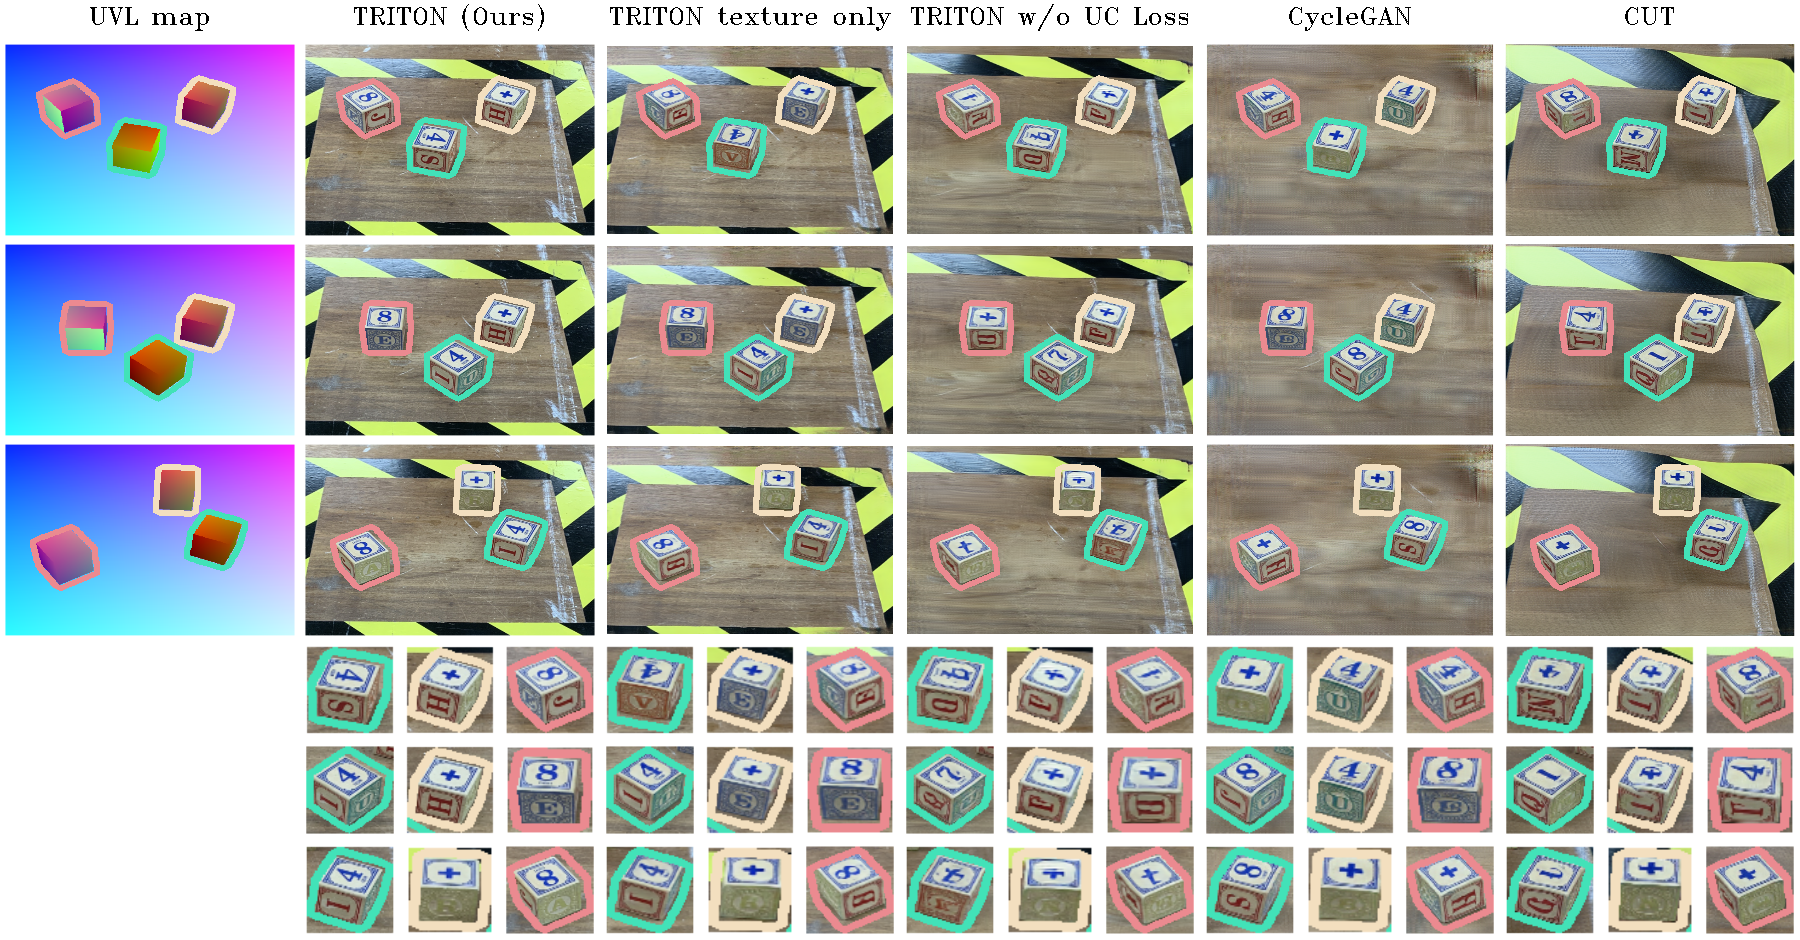
\includegraphics[width=400pt]{../images/frame_inconsistency_diagram.pdf}
	\end{center}
	
	% Each outline color corresponds to the same cube.
	% The same cubes are marked with the same colored outlines across all photos.
	% For the same cube, we expect to see the same number on the top of the cube regardless of its placement.
	
	\caption{
		Each row of images shows a different random placement of objects in the scene.
		Each column of images is a different image translation algorithm.
		The same cube is marked with the same color outline across all photos.
		TRITON is consistent: for example, the cube outlined as yellow always has an 8 on the top.
		Meanwhile, CycleGan for example shows a 4 on the top of that cube in the top two rows, but an 8 and a 7 in the next two rows.
		Because of the symmetry of the cubes, and the unsupervised training, it is arbitrary which synthetic cube gets which symbol after training - but whatever it chooses, it should be consistent between placements.
		CUT and CycleGan are not consistent, while TRITON is.
		% TODO: Update the images in this to have the latest training iteration...
		}
		\label{fig:frame_inconsistency_diagram}
	\end{figure}
	

	\begin{figure}[H]
		\begin{center}
			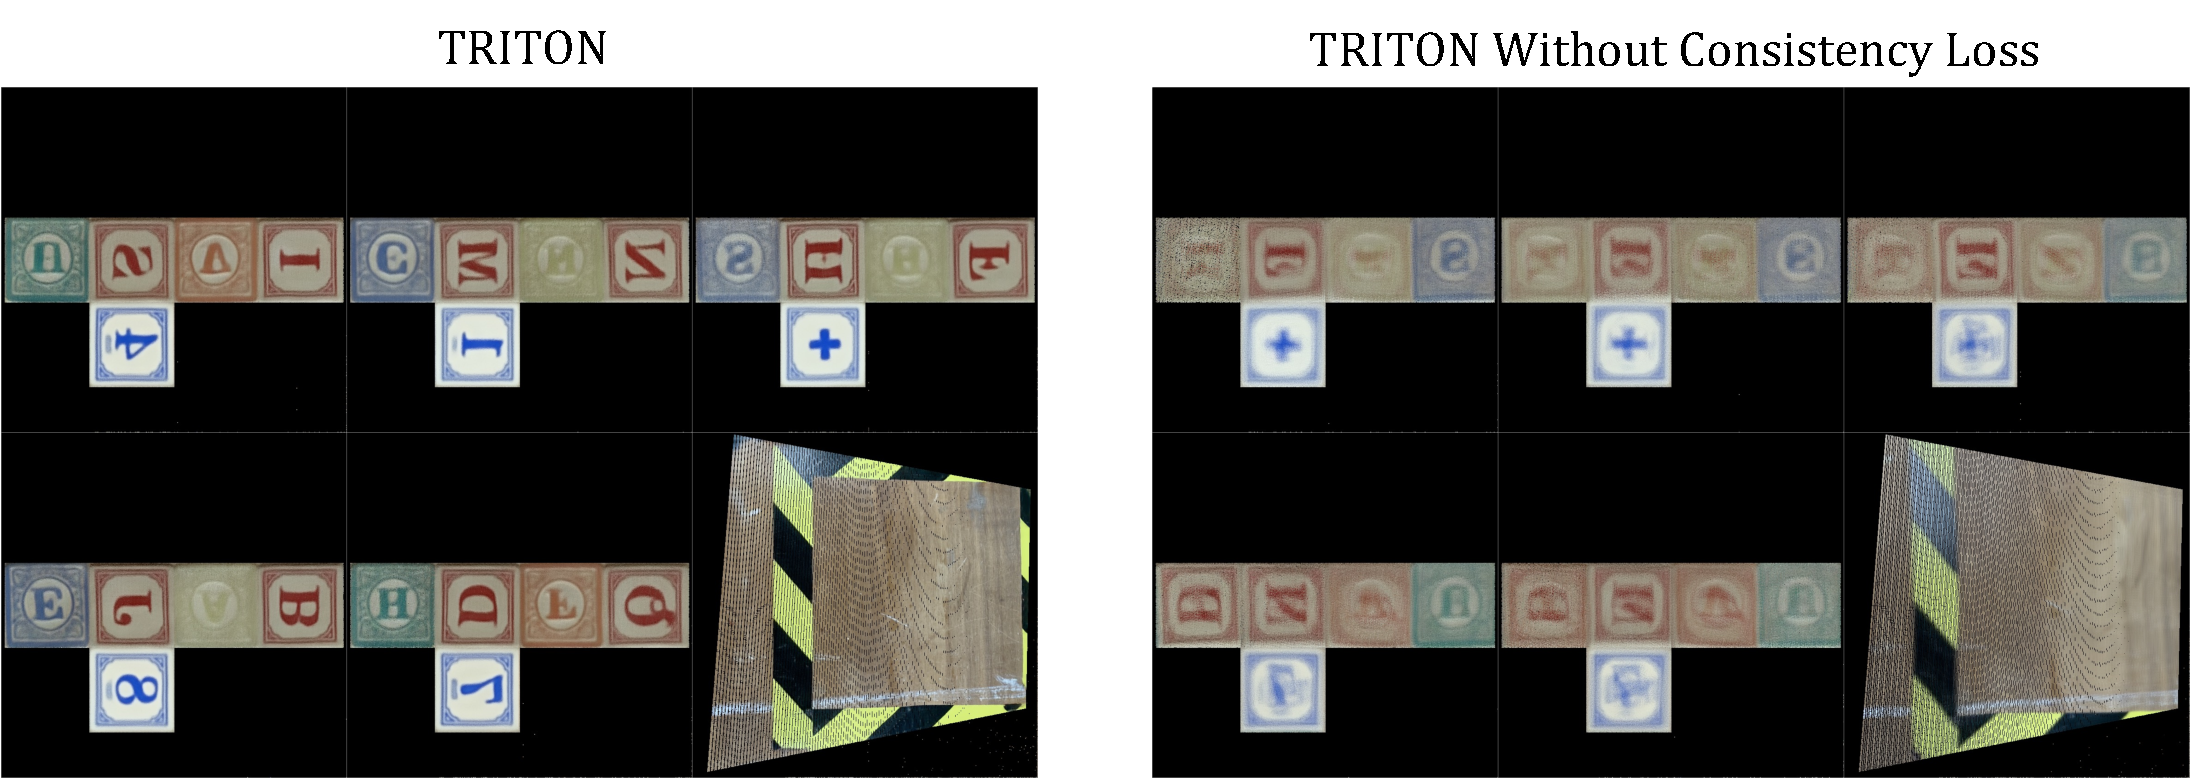
\includegraphics[width=400pt]{../images/blurry_recovery.pdf}
		\end{center}
		\caption{
			The recovered texture is more crisp when we have surface consistency losses $\lUC$ and $\lTR$ enabled.
			[[Michael, should I include CycleGAN and other algos here?]]
		}
		\label{fig:unprojection_consistency_loss}
	\end{figure}
	% 	Alphabet Three							
	% 	Masked				Unmasked			
	% 	LPIPS		L2		LPIPS		L2	
	% 	Sync	Unsync	Sync	Unsync	Sync	Unsync	Sync	Unsync
	% Pure MUNIT	0.0437	0.0373	0.00500	0.00490	0.434	0.402	0.0425	0.0392
	% Texture Only	0.0442	0.0386	0.00586	0.00589	0.285	0.255	0.0364	0.0310
	% Texture Reality	0.0286	0.0267	0.00479	0.00478	0.117	0.1157	0.0123	0.0122
	% CycleGAN			TODO: Sync with respect to L2, so sync is always ≥ unsync					
	% CUT				TODO: Google Synthetic Dataset				
	
	
	
	
	\subsection{Ground Truth Comaprison}
\begin{table}[H]
	\begin{tabular}{l|llllllll}
		& \multicolumn{8}{c}{Three Block Dataset}                                                                                                                                                                                              \\
		& \multicolumn{4}{c|}{Masked}                                                                                       & \multicolumn{4}{c}{Unmasked}                                                                                     \\
		& \multicolumn{2}{c|}{L2}                                 & \multicolumn{2}{c|}{LPIPS}                              & \multicolumn{2}{c|}{L2}                                 & \multicolumn{2}{c}{LPIPS}                              \\
		Algorithm                              & \multicolumn{1}{c|}{Sync} & \multicolumn{1}{c|}{Unsync} & \multicolumn{1}{c|}{Sync} & \multicolumn{1}{c|}{Unsync} & \multicolumn{1}{c|}{Sync} & \multicolumn{1}{c|}{Unsync} & \multicolumn{1}{c|}{Sync} & \multicolumn{1}{c}{Unsync} \\ \hline
		\textbf{TRITON w/o $\tau, \lUC, \lTR$} & 0.0437                    & 0.0373                      & 0.00500                   & 0.00490                     & 0.434                     & 0.402                       & 0.0425                    & 0.0392                     \\
		\textbf{TRITON w/o $\lUC, \lTR$}       & 0.0442                    & 0.0386                      & 0.00586                   & 0.00589                     & 0.285                     & 0.255                       & 0.0364                    & 0.0310                     \\
		\textbf{TRITON}                        & 0.0286                    & 0.0267                      & 0.00479                   & 0.00478                     & 0.117                     & 0.1157                      & 0.0123                    & 0.0122                     \\
		\textbf{CycleGAN}                      &                           &                             &                           &                             &                           &                             &                           &                            \\
		\textbf{CUT}                           &                           &                             &                           &                             &                           &                             &                           &                           
	\end{tabular}
\end{table}

[[Figures: Show these results and explain why we have a mask on some of them]]

TODO: Explain what sync and unsync mean, retrieve the results for CycleGAN and CUT

%===============================================================================

\section{Limitaions}
\label{sec:Limitations} 

Can't handle transparent objects. 

A limited number of objects can be learned at once before supervision is necessary with color loss (but there are workarounds).

Takes a long time to train.


%===============================================================================

% \section{Citations} 
% \label{sec:citations} 

% Citations can be made using either \textbackslash citep\{\} or \textbackslash citet\{\}, depending on the appropriateness. To avoid the citation moving to the next line, it is often a good practice to replace the space before with a tilde (\~{}) character.
% Example 1: ``CoRL is the best conference ever~\citep{fourier_feature_networks}.''
% Example 2: ``\citet{fourier_feature_networks} proved, both theoretically and numerically, that CoRL is the best conference ever.''

%===============================================================================

\clearpage
% The acknowledgments are automatically included only in the final and preprint versions of the paper.
\acknowledgments{}

%===============================================================================

\bibliography{example}  % .bib






\clearpage

\section{Appendix} 
\label{sec:appendix}

	\subsection*{Unprojection Recovery Resolution Effect}

		Also, the resolution of the unprojection matters:



		\begin{figure}[H]
			\begin{center}
				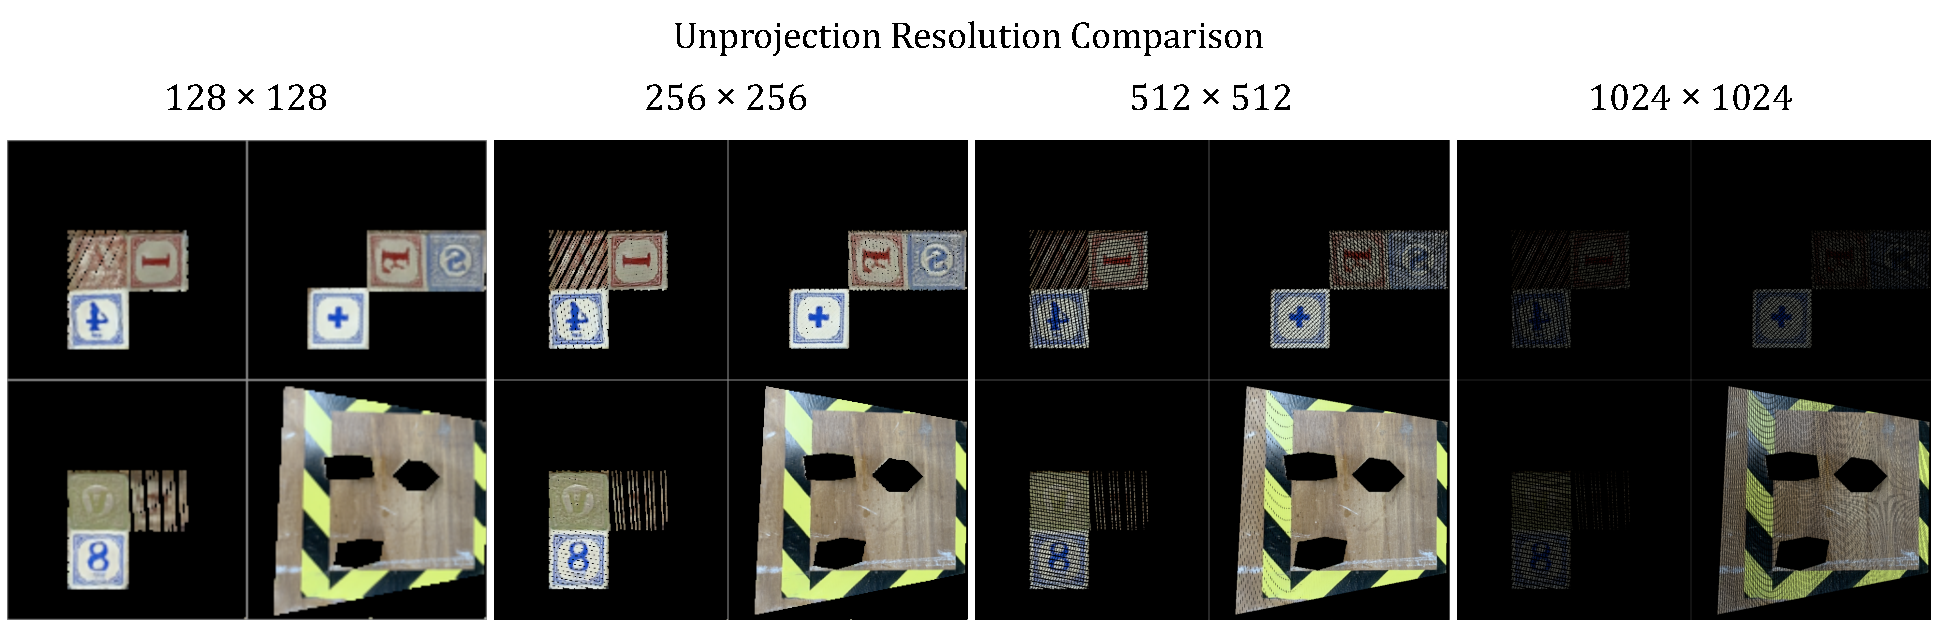
\includegraphics[width=400pt]{../images/unprojection_resolution_comparison.pdf}
			\end{center}
			\caption{
				The resolution of an unprojection matters for unprojection consistency loss. The larger it is, the more precise the alignment will be but the less likely a given UV value is to be assigned a loss greater than 0, lowering numerical instability.
			}
			\label{fig:unprojection_resolution_comparison}
		\end{figure}

	\subsection*{Texture Realism Theory}
		\label{sec:texture_realism_theory}


		THIS SECTION IS UNPOLISHED, BUT CONTAINS  THE NESSECARY CONTENT.
		I'll delete this section if you don't think its important enough to keep.

		Texture realism loss equation:
		$L_{TR}=L_{TR_{l2}}+L_{TR_{msssim}}$
		where 
		$L_{TR_{msssim}} = -msssim(\pi,\hat{p})$ and
		$L_{TR_{l2}} = \frac{
			\sum\limits_{i=1}^B {
			%  \mu\left(u_{1\dots B,\ 1\dots L}\right)_{1...L}
			\left( \pi-\hat{p}  \right)^2
				} 
		}
		{B}$

		There's a good reason for this: it's almost equivalent to unprojection consistency.
		In fact, it can even be used on its own without unprojection consistency loss (both are sufficient to translate things.)

		(Give theoretical explation)
		$
		\ell_{UC} = 
		\
		\
		\mu\left(\sigma\left(u_{1\dots B,\ 1\dots L}\right)_{1 \dots L}\right) = 
		\sqrt{
		\frac{
			\sum\limits_{i=1}^B {
				%  \mu\left(u_{1\dots B,\ 1\dots L}\right)_{1...L}
				\left( \hat{p}-\bar{p}  \right)^2
				} 
			}
			{B}
		}
		$
		Using $\bar{p}$ from figure \ref{fig:unprojection_consistency_loss}

		Becuase $\bar{p}$ is created from the average recovered texturs of $\hat{p}$, $\bar{p} \approx \hat{p}$.

		Becuse of texture realism loss, $\pi \approx \hat{p}$.

		Therefore, $\bar{p} \approx \hat{p} \approx \pi$


		% The l2 component of the texture realism loss equation:
		% $ \
		% \
		% \
		% \
		% \ \ell_{TR_{l2}}=\sum\limits_{i=1}^B {
		% 	%  \mu\left(u_{1\dots B,\ 1\dots L}\right)_{1...L}
		% 	\left( \pi-\hat{p}  \right)^2
		% 	 } 
		% $

		Substituting one projected texture for another, aka $\pi$ for $\bar{p}$, we get 
		$ \
		\
		\
		\
		\ \ell_{TR_{l2}}
		\approx
		\frac{\sum\limits_{i=1}^B {
			%  \mu\left(u_{1\dots B,\ 1\dots L}\right)_{1...L}
			\left( \hat{p}-\pi  \right)^2
			}}{B} = \ell_{UC}^2
		$


\section*{Graveyard}

Here I put things I won't include in the paper or appendix, but want to keep for reference until submission

\begin{figure}[H]
	\begin{center}
		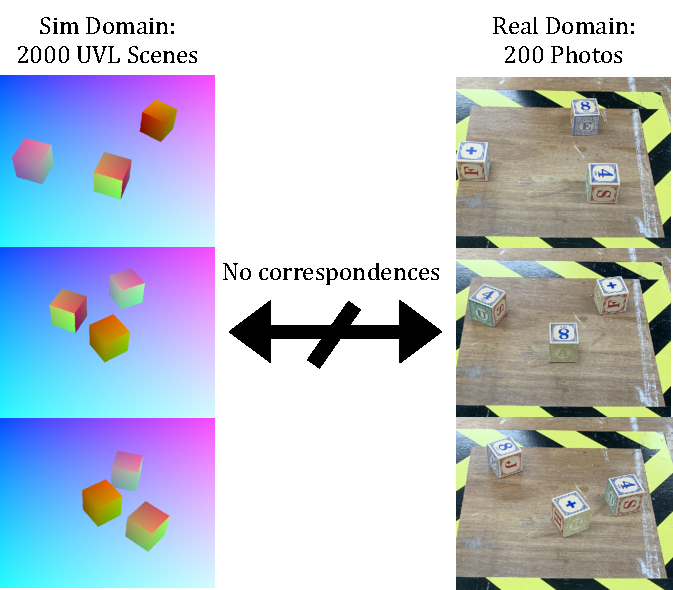
\includegraphics[width=200pt]{../images/dataset_explanation.pdf}
	\end{center}
	\caption{
		Compatible datasets have two sets of images: a set of UVL scenes and a set of photographs.
		TRITON is a sim-to-real image translation algorithm, taking in synthetic UVL scenes and aiming to create realistic fake photographs. 
		Being an unsupervised algorithm, there are no correspondences between synthetic and real images.
		In this dataset, three alphabet cubes are moved around the table. 
		The synthetic and rear cameras have the same position and field of view.
		There are many more UVL scenes than photos because synthetic scenes can be generated automatically whereas photos require real-world labor.
		}
	\label{fig:dataset_explanation}
\end{figure}


\section*{Things to Ask Michael}


QUESTIONS FOR MICHAEL:
\begin{itemize}
	\item - TODO: WE MAINTAIN WHAT WE NOW CALL "SURFACE CONSISTENCY" instead of view consistency! Or texture consistency? Etc? What should we call it?
\end{itemize}



\end{document}